\documentclass[11pt,a4paper]{article}
\usepackage[utf8]{inputenc}
\usepackage{amsmath}
\usepackage{amsfonts}
\usepackage{amssymb}
\usepackage{graphicx}
\usepackage{hyperref}
\usepackage{cite}
\usepackage{minted}
\renewcommand{\baselinestretch}{1.5}

\author{Clara Maier, Nico Fröhlich}
\title{Seminarkurs - Alan Turing}

\begin{document}
\maketitle
\newpage
\tableofcontents
\newpage
\emph{Hiermit versichern wir, die vorliegende Arbeit selbstständig und nur unter Zuhilfenahme der angegeben Quellen und Hilfsmittel angefertigt zu haben. Aus den angegebenen Materialien entnommene Inhalte und Zitate sind als solche kenntlich gemacht. Wir erklären, dass wir zu diesem Thema nicht schon einmal eine solche Arbeit angefertigt habe.}
\newpage
\section{Vorwort}
Der Vater des Computer, die Person die wahrscheinlich den zweiten Weltkrieg um zwei Jahre verkürzte, was gibt es da noch zu sagen? Alan Turing eine der bekanntesten und einflussreichsten Mathematiker des letzten Jahrhunderts. Er beeinflusst nicht nur die Mathematik und heutige Informationstechnik, durch die Turingmaschine zum Beispiel, sondern auch die Philosophie, durch zum Beispiel den Turing Test. In seinem meist Zitierten Papier ging es sogar um Biologie. Am bekanntesten, nicht zuletzt durch den Film 'the imitation game', ist jedoch seine Beteiligung am zweiten Weltkrieg, durch die Entschlüsselung der Enigma der Nazis. Seine Arbeit im Bereich Computer Technik sowie in Ethik, Philosophie, sein Papier über Maschinen und Intelligenz sind mehr als nur Interessant. Sie sind weit mehr als das. Turing hat mit diesen Werken unsere heutiges Leben maßgeblich beeinflusst. In den Folgenden Kapiteln wird die tragische Geschichte rund um Alan Turing und ein paar seiner Zeitgenossen beleuchtet. Die Turing Maschine der Turing Test und seine Auswirkungen auf die Zukunft, sowie die Turing-Church-Hypothese werden in den Folgenden Abschnitten beleuchtet.
\section{Historie}
Alan Mathison Turing wurde 1912, am 23 Juni in London geboren. Er starb am 7 Juni 1954 im Alter von 42 Jahren an seinem Wohnort in Wilmslow in Cheshire.
Seine Eltern Ethel und Julius Turing sind für seine Geburt  
\section{Turing Maschine}
Die Turingmaschine wurde 1936 von Alan Turing entwickelt und ist rein theoretisch, denn eine Maschine exakt wie es Turing beschreibt wurde niemals gebaut, da dies auch nicht sinnvoll wäre. Turing entwickelte diese Theorie aufrund des Entscheidungsproblem von David Hilber und Wilhelm Ackermann \cite{theessentialturing}. Die Turing Maschine ist die heutige Grundlage vieler Programmiersprachen, wie Java, C++ oder Phyton. Diese Programmiersprachen werden auch als Turing complete bezeichnet, was so viel heißt wie dass die Turing Maschine diese theoretischer weiße emulieren kann.

\subsection{Funktion} 
Die Turing Maschine beinhaltet lediglich zwei Bauteile.
\begin{enumerate}
\item  Ein unendlich langes Band, dass in eine Kette von horizontalen Kästchen eingteilt ist. Jedes dieser Kästchen kann entweder eine 0,eine 1 oder auch nichts beinhalten. Zudem kann das Band nach rechts und nach links verschoben werden.
\item Ein Kasten auch "Heap" genannt, der die Zahlen auf dem Band einlesen,löschen und ändern kann.
\end{enumerate}
 


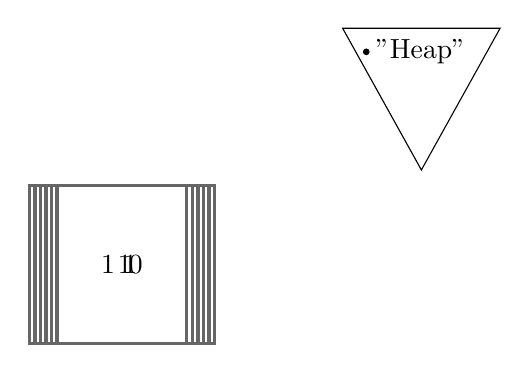
\begin{tikzpicture}[
squarednode/.style={rectangle, draw=black!60, very thick, minimum size=20mm}
]
%Nodes
\node[squarednode][right=0] {1};
\node[squarednode][right=2]{ };
\node[squarednode][right=4]{ };
\node[squarednode][right=6]{1};
\node[squarednode][right=8]{1};
\node[squarednode][right=10]{0};
 
%Lines
\draw[black](4,3) -- (5,1.2) -- (6,3) -- cycle;
\filldraw[black] (4.3,2.7) circle (1pt) node[anchor=west] {"Heap"}; %??????


\end{tikzpicture}



\subsection{Beispiel} Zur besseren Vorstellung, erkläre ich das Ganze nochmal an einem Beispiel. Nehmen wir mal an wir wollen, dass die Turing Maschine für uns unendlich Hochzählt. So kann man dies mit nur zwei einfachen Befehlen ausführen. 

\begin{itemize}
\item Befehl 1 = Bei einer 1, ändere diese in eine 0 und gehe nach links 
\item Befehl 2 = Bei einer 0 oder einer Lücke, ändere diese in eine 1 und gehe zum letzten Bit der Zahl 
\end{itemize}

Die Befehle für die Turing Maschine kann man sich also heute wie die Programme auf unseren Computern vorstellen.
\section{Lambda calculus}
Der Lambda calculus ist ein Datenverarbeitungskonzept erfunden von Alonzo Church, dem Professor von Alan Turing. Turing studierte unter Church einige Zeit an der Princeton Universität bevor er dann wieder zurück nach England ging. Im folgenden Abschnitt wird kurz auf Church eingegangen, danach wird Churches Werk, der Lambda calculus, dessen Gesetze, Notation und Beispiele behandelt. Hier wird ein Einblick in die Welt der funktionellen Programmiersprachen und ihrer Geschichte gegeben.
\subsection{Alonzo Church}
\subsection{Gesetze des Lambda calculus}
Der Lambda calculus besteht aus 3 Grundgesetzen.
\begin{itemize}
\item Funktionen können erstellt werden.
\item diese können/müssen Daten Ein und Ausgeben.
\item Man weiß nicht was die Funktionen tun.
\end{itemize}
Ausführlicher: Es muss ein Weg vorhanden sein eine Funktion zu definieren, dafür gibt es eine Mathematische Definition. Die Erzeugung einer Funktion ist aber nicht auf die Mathematische Notation beschränkt, ganz im Gegenteil, die Notationen im Modernen Lambda Programming weichen, nicht zuletzt aus technischen Gründen, stark von der Mathematischen Notation ab. Dabei müssen im originalen Lambda Ein- und Ausgaben definiert werden. Dies weicht im modernen Lambda ebenfalls von der originalen Definition ab. Hier können Ein- und Ausgaben definiert werden, müssen es aber nicht. Dies führt zu mehr Flexibilität, so können die Lambda Funktionen auch an stellen Eingesetzt werden wo nicht direkt Daten verarbeitet werden. Als letztes kennt man beim Ausführen der Funktion den Inhalt der Funktion nicht. Das ist der große unterschied zu anderen Mathematischen Funktionen.\cite{lambdacalculus}
\subsection{Lambda in Programmiersprachen}
Schauen wir uns zur Erläuterung ein Beispiel aus Java an.
Es gibt eine Funktionsdeklaration die der Implementation vorgibt welche Ein und Ausgänge
eine gewisse Lambda Funktion hat sowie ihren Namen.
\begin{minted}{java}
@FunctionalInterface
public interface TestFunctionalInterface {
	public int test(double d);
}
\end{minted}
Die Funktion wird nun als Interface übergeben und von einer ausführenden Funktion genutzt.
Was hier auffällt ist das die ausführende Funktion nicht weiß was die Funktion eigentlich tut.
\begin{minted}{java}
public void runTest(TestFunctionalInterface interf) {
	int testres = interf.test(89.1);
	// Mache etwas mit dem resultat
}
\end{minted}
Normalerweise müsste man dieses Interface überschreiben und dort dann implementieren was die Funktion tun würde. Hier gibt es allerdings eine separate schreib weise um eine Funktion zu definieren. Die wie folgt durch die Zeichen Kombination -> eingeleitet wird.
Rechts von dem sog. Lambda operator stehen die Inputs rechts die Operationen bzw. Outputs 
\begin{minted}{java}
public void main() {
	runTest(input -> (int)Math.ceil(input));
}
\end{minted}

\subsection{Mathematische Notation}
Für den Ursprünglichen Lambda calculus definiert von Alonzo Church gibt es auch eine Mathematische Notation die wie Folgt durch das Zeichen Lambda eingeleitet wird.
\begin{equation}
\lambda(x) = x * 2
\end{equation}
Die Ursprüngliche Notation ist weit aus Mathematischer als die in derzeitigen Programmiersprachen. Dennoch lassen sich damit beliebig Daten verarbeiten. .\cite{lambdacalculus}
\begin{equation}
\lambda
\end{equation}
So lässt sich z.B. ein boolean wert (also true/false oder 1/0) verarbeiten 
\footnote{Kapitel 4 von Nico}
\section{Church-Turing Thesis}
In diesem Kapitel geht es um die Church-Turing Thesis, was sie besagt und was für Auswirkungen sie hat. Außerdem wird im Zuge dessen die Turing Maschine und der Lambda calculus gegenübergestellt.
\subsection{Die These}
Die These besagt, dass alle möglichen Rechnungen bzw. Datenverarbeitungen mit dem Modell der Turing Maschine dargestellt werden können. Des weiteren ist der Lambda calculus mit der Turing Maschine gleich zu stellen, das heißt, dass ebenfalls alle 
\cite{sep-church-turing}
\section{Turingtest}
\label{turingtest}
In diesem Abschnitt geht es um Turings Ausflug in die Philosophie und sein Werk "Computing Machinery and Intelligence". Dabei wird die Frage betrachtet ob Maschinen denken können und wie man eine Maschine von einen Menschen unterscheiden kann. Sowie heutige Anwendungen und Auswirkungen auf Kunst und Gesellschaft.
\subsection{The Imitation Game}
Turing stellt eine bessere Frage in den Raum, als die Frage "Können Maschinen Denken?". Um die Frage allerdings stellen zu können muss ich das "Imitation Game" einführen. Das Spiel funktioniert wie folgt. Lass A ein Mann sein, B eine Frau und C einen Detektiv. Der Detektiv (C) will also heraus finden wer welches Geschlecht hat, ohne dabei die Sprache zu hören oder die Person zu sehen. Um diesen Zustand zu gewährleisten gehen wir davon aus, dass der Detektiv in einem anderen Raum ist wie A und B, die einzige Kommunikation die besteht ist also textbasiert. Also versucht C Fragen zu verwenden, um mit Hilfe der Antworten beider Personen zu bestimmen, welche weiblich und welcher männlich ist. Dies wendet Turing nun auf Maschinen an, dabei beschränkt er sich auf Digitalcomputer. Es wird versucht auf äußerliche Fragen zu verzichten, da dies zu keinem eindeutigen Ergebnis führen würde. Die Maschine könnte ganz einfach ein eigenes fingiertes Aussehen annehmen und die Person kennt ihres, daher ist es schwierig anhand der Antworten eindeutig zu unterscheiden. Deshalb versucht C logische Fragen zu verwenden um heraus zu finden ob es sich um eine reale Person handelt. Beispiel: Subtrahiere 56 von 18934.\cite{computing} Dieses Spiel wird nun nicht nur dazu genutzt eine Maschine von einem Menschen zu unterscheiden, sondern es wird implizit die Frage gestellt ob eine Maschine denken kann. Wenn man ihre Antworten nämlich nicht mehr voneinander unterscheiden kann, muss man sich Gedanken darüber mache,  ob wir dann nicht intelligentes Leben geschaffen haben könnten und wie wir dieses dann behandeln.
\subsection{Chinese room problem}
Eine der berühmtesten Probleme des Turing Tests ist das chinese room problem. Dieses Problem stellt in Frage, ob man mit dem Turingtest wirklich die Intelligenz eines Lebewesens feststellen kann. Dabei wird eine weitere Situation angenommen. Nehmen wir also an zwei Personen sitzen sich gegenüber in einem Raum. Die eine Person ist ein Chinese die andere Person ein Deutscher. Auf dem Tisch liegt nun ein Deutsch-Chinesisch Wörterbuch. Die beiden Personen versuchen miteinander zu kommunizieren. Dazu nutzt der Deutsche ein Wörterbuch. Nun stellt sich die Frage, wenn der Deutsche nun seinen Satz auf Chinesisch übersetzt, ob er wirklich weiß was er sagt. Übertragen auf eine Maschine stellt sich nun ebenfalls die Frage, kann die Maschine wirklich wissen was sie tut und diese Aktionen auch selber hinterfragen. Darüber hinaus stellt sich die Frage wie intelligent Maschinen wirklich werden können.
\subsection{Anwendungen in der Moderne}
Hier folgt eine kurze Beleuchtung des heutigen Einsatzfeldes des Turing Tests. Dieser wird in der Internetsicherheit sehr oft verwendet um automatisierte Anfragen zu filtern. Als Beispiel wird hier exemplarisch ReCaptcha von Google beleuchtet. Es gibt aber genug andere sogenannte Captcha Methoden. Diese geben eine Art von Frage an, hierbei ist die Kommunikation allerdings nicht nur wie im Turing Test, auf textbasierte Kommunikation beschränkt. Im Gegenteil, hier werden sogar bewusst Bilder eingesetzt, damit der zu testende Computer beziehungsweise die Person die den Computer bedient, eine Frage zu diesen Bildern beantworten muss. Dabei sind die Antworten auf die eigentliche Frage nicht einmal so wichtig wie es einem im ersten Moment erscheint. Die Ironie, und eine weitere Abweichung ist dabei, dass man hier gegen ein neuronales Netzwerk "spielt". Dieses muss anhand der vorliegenden Informationen bestimmen, ob die Anfrage von einem Mensch stammt oder ob es sich dabei nur um eine automatisch generierte Anfrage handelt. Wie genau dieses Netzwerk entscheidet weiß wahrscheinlich nicht mal Google. Wichtig ist aber welche Daten dem Netzwerk dabei zur Verfügung gestellt werden, um seine Entscheidung zu treffen. Für weitere Informationen verweise ich hier auf einen Blog-Eintrag\cite{captcha}. Zu den auszuwertenden Daten gehören unter anderem die Mausbewegungen sowie die gesendeten Daten des Browsers (z.B. User-Agent, IP, Cookies).
\subsection{Auswirkungen auf Kunst und Gesellschaft}
Diese grundsätzlichen Gedanken und die Frage, ob Maschinen überhaupt denken können hat weitreichende Auswirkung auf die Moderne Kunst, darunter vor allem Computerspiele. Sehr gute Beispiele sind, das gleichnamige Spiel "The Turing Test" oder auch "The Talos Principle" in denen der Turing Test sehr häufig vorkommt. Es ist wichtig hier darauf aufmerksam zu machen, dass das Imitation Game heute noch für sehr viel Kopfzerbrechen unter den Wissenschaftlern, Philosophen so
wie in der gesamten Gesellschaft auslöst. Wir werden bald an den Zeitpunkt kommen wo es wichtig sein wird, sich mit dieser Frage auseinander zu setzen. Weiterführend dazu siehe The future of the mind: Exploring machine consciousness von Dr. Susan Schneider\cite{explorecons}



\bibliography{main}
\bibliographystyle{ieeetr}

\end{document}